% Bagian: model-theory
% Bab: interpolation
% Subbagian: separation

\documentclass[../../../include/open-logic-section]{subfiles}

\begin{document}

\olfileid[id]{mod}{int}{sep}

\olsection{Pemisahan \printtoken{P}{sentence}}

Kita memerlukan sedikit persiapan sebelum melanjutkan ke bukti teorema
interpolasi. Interpolan bagi $!A$ dan $!B$ adalah !!a{sentence}~$!C$
sedemikian sehingga $!A \Entails !C$ dan $!C \Entails !B$. Dengan
kontraposisi, yang terakhir berlaku jika dan hanya jika $\lnot !B \Entails
\lnot !C$. !!^a{sentence}~$!C$ dengan sifat ini dikatakan
\emph{memisahkan} $!A$ dan $\lnot !B$. Jadi, mencari interpolan bagi $!A$
dan $!B$ sama dengan mencari !!a{sentence} yang memisahkan $!A$ dan
$\lnot !B$. Seperti sering terjadi, akan berguna untuk meninjau suatu
generalisasi: kalimat yang memisahkan dua \emph{himpunan} !!{sentence}s.

\begin{defn}
Suatu kalimat $!C$ \emph{memisahkan} himpunan kalimat $\Gamma$ dan
$\Delta$ jika dan hanya jika $\Gamma \Entails !C$ dan $\Delta \Entails
\lnot !C$. Jika tidak ada !!{sentence} semacam itu, maka $\Gamma$ dan
$\Delta$ \emph{tidak terpisahkan}.
\end{defn}

Relasi inklusi antara kelas-kelas model dari $\Gamma$, $\Delta$, dan $!C$
digambarkan di bawah ini:
\begin{figure}[h]
  \centering
  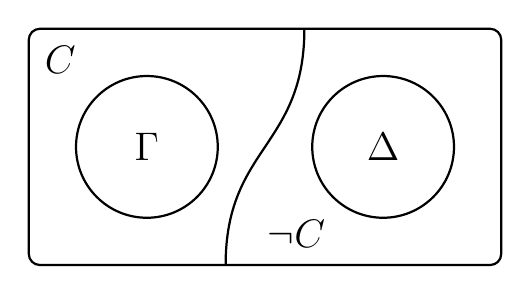
\begin{tikzpicture}[node distance=2cm, auto, thick]
    \draw [rounded corners] (0,0) -- (6,0) -- (6,3) -- (0,3) --  cycle;
    \draw (1.5,1.5) circle (0.9cm);
    \draw (4.5,1.5) circle (0.9cm);
    \path node at (1.5,1.5) {\Large $\Gamma$};
    \path node at (4.5,1.5) {\Large $\Delta$};
    \path node at (0.4,2.6) {\Large $\formula{C}$};
    \path node at (3.4,0.4) {\Large $\lnot \formula{C}$};
    \draw (2.5,0) .. controls (2.5,1.5) and (3.5,1.5) .. (3.5,3);
  \end{tikzpicture}
  \caption{$!C$ memisahkan $\Gamma$ dan $\Delta$}
  \ollabel{fig:sep}
\end{figure}


\begin{lem}\ollabel{lem:sep1}
Andaikan $\Lang{L}_0$ adalah bahasa yang memuat setiap !!{constant},
!!{function}, dan !!{predicate} (selain $\doteq$) yang terdapat dalam
\emph{keduanya}, $\Gamma$ dan $\Delta$, dan misalkan $\Lang{L}'_0$
diperoleh dengan menambahkan tak hingga banyak !!{constant} baru $\Obj c_n$
untuk $n \ge 0$. Jika $\Gamma$ dan $\Delta$ tidak terpisahkan dalam
$\Lang{L}_0$, maka keduanya juga tidak terpisahkan dalam $\Lang{L}'_0$.
\end{lem}

\begin{proof}
Kita menggunakan pembuktian tak langsung: andaikan, demi memperoleh
kontradiksi, bahwa $\Gamma$ dan $\Delta$ terpisahkan dalam $\Lang{L}'_0$.
Maka $\Gamma \Entails \Subst{!C}{c}{x}$ dan $\Delta \Entails \lnot
\Subst{!C}{c}{x}$ bagi suatu $!C \in \Lang{L}_0$ (dengan $c$ suatu
!!{constant} baru---kasus ketika $!C$ memuat lebih dari satu !!{constant}
baru semacam itu serupa). Menurut kekompakan, terdapat himpunan bagian
\emph{hingga} $\Gamma_0$ dari $\Gamma$ dan $\Delta_0$ dari $\Delta$
sedemikian sehingga $\Gamma_0 \Entails \Subst{!C}{c}{x}$ dan
$\Delta_0 \Entails \lnot \Subst{!C}{c}{x}$. Misalkan $!G$ konjungsi
semua !!{formula}s dalam $\Gamma_0$ dan $!H$ konjungsi semua !!{formula}s
dalam $\Delta_0$. Maka
\begin{align*}
  !G & \Entails \Subst{!C}{c}{x}, & !H  \Entails \lnot \Subst{!C}{c}{x}.
\end{align*}
Dari yang pertama, melalui Generalisasi, kita memperoleh $!G \Entails
\lforall[x][!C]$; dari yang kedua, melalui kontraposisi,
$\Subst{!C}{c}{x} \Entails \lnot !H$, sehingga juga $\lforall[x][!C]
\Entails \lnot !H$. Kontraposisi sekali lagi memberikan $!H \Entails
\lnot \lforall[x][!C]$. Menurut monotonisitas,
\begin{align*}
  \Gamma &\Entails \lforall[x][!C], &
  \Delta & \Entails \lnot \lforall[x][!C],
\end{align*}
sehingga $\lforall[x][!C]$ memisahkan $\Gamma$ dan $\Delta$ dalam
$\Lang{L}_0$.
\end{proof}

\begin{lem}\ollabel{lem:sep2}
Andaikan $\Gamma \cup \{ \lexists[x][!S] \}$ dan $\Delta$ tidak
terpisahkan, dan $c$ adalah !!{constant} baru yang tidak terdapat dalam
$\Gamma$, $\Delta$, ataupun $!S$. Maka $\Gamma \cup \{
\lexists[x][!S], \Subst{!S}{c}{x} \}$ dan $\Delta$ juga tidak
terpisahkan.
\end{lem}

\begin{proof}
Andaikan, demi memperoleh kontradiksi, bahwa $!C$ memisahkan $\Gamma \cup
\{\lexists[x][!S], \Subst{!S}{c}{x}\}$ dan $\Delta$, sementara
$\Gamma \cup \{\lexists[x]{!S} \}$ dan $\Delta$ tidak terpisahkan.
Kita membedakan dua kasus:
\begin{enumerate}
\item $c$ tidak terdapat dalam $!C$: dalam hal ini $\Gamma \cup
  \{\lexists[x][!S], \lnot!C \}$ dapat dipenuhi (jika tidak, $!C$
  memisahkan $\Gamma \cup \{\lexists[x][!S] \}$ dan $\Delta$).
  Himpunan itu tetap dapat dipenuhi setelah $\Subst{!S}{c}{x}$
  ditambahkan, sehingga pada akhirnya $!C$ tidak memisahkan $\Gamma \cup
  \{ \lexists[x][!S], \Subst{!S}{c}{x} \}$ dan $\Delta$.
\item $c$ terdapat dalam $!C$, sehingga $!C$ berbentuk
  $\Subst{!C}{c}{x}$. Maka kita mempunyai
  \[
  \Gamma \cup \{ \lexists[x][!S], \Subst{!S}{c}{x}\} \Entails \Subst{!C}{c}{x},
  \]
  sehingga $\Gamma, \lexists[x][!S] \Entails \lforall[x][(!S \lif !C)]$
  menurut Teorema Deduksi dan Generalisasi, dan akhirnya $\Gamma
  \cup \{ \lexists[x][!S] \} \Entails \lexists[x][!C]$. Di sisi lain,
  $\Delta \Entails \lnot \Subst{!C}{c}{x}$ dan karenanya, menurut
  Generalisasi, $\Delta \Entails \lnot \lexists[x][!C]$. Jadi $\Gamma
  \cup \{\lexists[x][!S] \}$ dan $\Delta$ terpisahkan, suatu
  kontradiksi.
\end{enumerate}
\end{proof}

\end{document}
